\documentclass{article}\usepackage{graphicx, color}
%% maxwidth is the original width if it is less than linewidth
%% otherwise use linewidth (to make sure the graphics do not exceed the margin)
\makeatletter
\def\maxwidth{ %
  \ifdim\Gin@nat@width>\linewidth
    \linewidth
  \else
    \Gin@nat@width
  \fi
}
\makeatother

\IfFileExists{upquote.sty}{\usepackage{upquote}}{}
\definecolor{fgcolor}{rgb}{0.2, 0.2, 0.2}
\newcommand{\hlnumber}[1]{\textcolor[rgb]{0,0,0}{#1}}%
\newcommand{\hlfunctioncall}[1]{\textcolor[rgb]{0.501960784313725,0,0.329411764705882}{\textbf{#1}}}%
\newcommand{\hlstring}[1]{\textcolor[rgb]{0.6,0.6,1}{#1}}%
\newcommand{\hlkeyword}[1]{\textcolor[rgb]{0,0,0}{\textbf{#1}}}%
\newcommand{\hlargument}[1]{\textcolor[rgb]{0.690196078431373,0.250980392156863,0.0196078431372549}{#1}}%
\newcommand{\hlcomment}[1]{\textcolor[rgb]{0.180392156862745,0.6,0.341176470588235}{#1}}%
\newcommand{\hlroxygencomment}[1]{\textcolor[rgb]{0.43921568627451,0.47843137254902,0.701960784313725}{#1}}%
\newcommand{\hlformalargs}[1]{\textcolor[rgb]{0.690196078431373,0.250980392156863,0.0196078431372549}{#1}}%
\newcommand{\hleqformalargs}[1]{\textcolor[rgb]{0.690196078431373,0.250980392156863,0.0196078431372549}{#1}}%
\newcommand{\hlassignement}[1]{\textcolor[rgb]{0,0,0}{\textbf{#1}}}%
\newcommand{\hlpackage}[1]{\textcolor[rgb]{0.588235294117647,0.709803921568627,0.145098039215686}{#1}}%
\newcommand{\hlslot}[1]{\textit{#1}}%
\newcommand{\hlsymbol}[1]{\textcolor[rgb]{0,0,0}{#1}}%
\newcommand{\hlprompt}[1]{\textcolor[rgb]{0.2,0.2,0.2}{#1}}%

\usepackage{framed}
\makeatletter
\newenvironment{kframe}{%
 \def\at@end@of@kframe{}%
 \ifinner\ifhmode%
  \def\at@end@of@kframe{\end{minipage}}%
  \begin{minipage}{\columnwidth}%
 \fi\fi%
 \def\FrameCommand##1{\hskip\@totalleftmargin \hskip-\fboxsep
 \colorbox{shadecolor}{##1}\hskip-\fboxsep
     % There is no \\@totalrightmargin, so:
     \hskip-\linewidth \hskip-\@totalleftmargin \hskip\columnwidth}%
 \MakeFramed {\advance\hsize-\width
   \@totalleftmargin\z@ \linewidth\hsize
   \@setminipage}}%
 {\par\unskip\endMakeFramed%
 \at@end@of@kframe}
\makeatother

\definecolor{shadecolor}{rgb}{.97, .97, .97}
\definecolor{messagecolor}{rgb}{0, 0, 0}
\definecolor{warningcolor}{rgb}{1, 0, 1}
\definecolor{errorcolor}{rgb}{1, 0, 0}
\newenvironment{knitrout}{}{} % an empty environment to be redefined in TeX

\usepackage{alltt}
\usepackage{url}
\usepackage{graphicx}
\usepackage{caption}
\usepackage{enumerate}
\usepackage{float}
\title{Global Temperature Anomalies}
\author{Geoffrey Thompson and Sam Benidt}
\date{12/14/2012}
\begin{document}


\maketitle




\begin{figure}[H]
\begin{knitrout}
\definecolor{shadecolor}{rgb}{0.969, 0.969, 0.969}\color{fgcolor}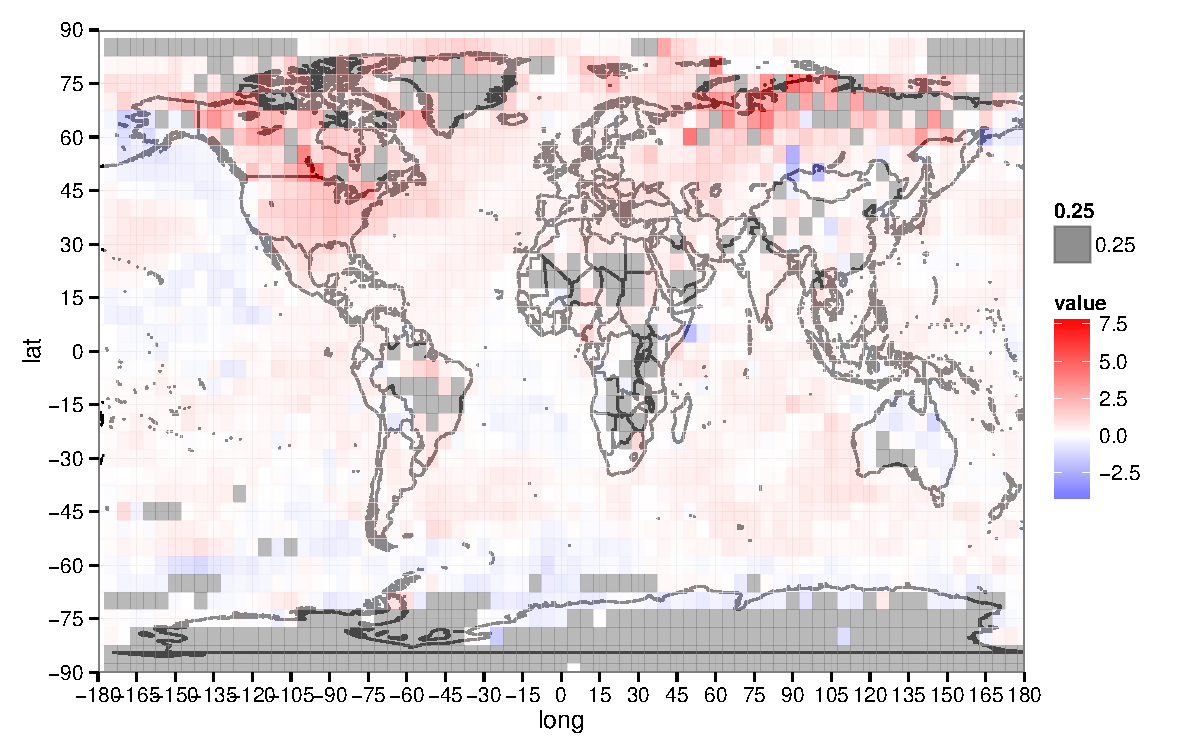
\includegraphics[width=\linewidth]{figure/recent-map} 
\end{knitrout}

\caption{\label{sep2012map}Map of temperature anomalies for September 2012}
\end{figure}

\section{Introduction}

The consensus of climate scientists is that the world has been warming since the Industrial Revolution and that it has been warming faster over the last several decades. The warming is not uniform - the poles are in general are warming much faster than the tropics. The rate of warming has also not been been increasing at a uniform rate over time. For example, the twenty periods from 1925-1944 and from 1978-1997 have seen the largest increases in temperature throughout the period of the twentieth century. We will be analyzing the HADCRUT4 temperature dataset which has a monthly record of temperature anomalies from a respective 1960-1991 baseline on a $5^{\circ}$ by $5^{\circ}$ gridded basis going back to 1850.  Using this dataset we will graphically explore when and where temperatures have been changing and by how much over the past 162 years. The HADCRUT4 dataset was the subject of some controversy in October when a journalist claimed the data showed no increase in temperature over the last 16 years (1997-2012). We will also attempt to graphically look further into this claim.

\section{Description of Data and Source:}
We pulled data on temperature deviations from a 1961 to 1990 temperature trend from the HADCRUT4 near surface temperature data set found at: \url{http://www.metoffice.gov.uk/hadobs/hadcrut4/data/current/download.html}.\\ This data is hosted by the Met Office Hadley Centre. The HADCRUT4 dataset combines data from the  CRUTEM4 and HadSST3 which contain data based on surface air temperature and sea-surface temperature respectively. The data is reported in 100 ensembles. We chose to look at the first ensemble dataset, which was a choice on convenience due to the large nature of each individual ensemble dataset. However, we hope that the same type of analysis recorded here could be used and would be applicable on any of the 100 ensembles.  The Global temperature trend was also downloaded which is computed from average of the Northern and Southern Hemispheres ((NH +SH)/2).

\section{Data Cleaning/Formatting:}
The temperature deviation data for ensemble 1 was downloaded in a spaced delimited ASCII file.  The ASCII file was opened up in Microsoft Excel and parsed to create a CSV file that contained meta data for the first month of 1850 on the first row followed by 36 rows and 72 columns of temperature deviations where the entry in row i and column j represented a measurement of temperature deviation for each latitude and longitude. This was followed by another row of metadata describing the second month of 1850 following by the same 36 rows by 72 columns of temperature deviations and so on. The CSV file was read into R. Each 37th row was deleted (including the first row) since those rows contained meta data. The variables time (in months since 1850), xloc, months (month of year), year(years since 1850). The data were reshaped to using the melt function keeping the variables time, xloc, months, year, and temp, allowing the yloc variable to be formed.  The variables real year and latitude and longitude were introduced to the data set through an appropriate transformation of the variables $year$, $xloc$, and $yloc$.

Global montly temperature deviation data was downloaded as well. However, there was not much work needed to put the data into a useable format.

\section{Main Section:}
\subsection*{Increased World Coverage}
The data are a worldwide data set spanning from 1850 to the present, but large portions of the world were still unexplored. The first explorer only set foot on Antarctica in 1840 (or 1821, depending on which account you believe) and reached the south pole in 1911. Whether or not a spot has a set of temperature records in a given year indicates whether scientific meteorology has made it there. In 1850, the records were spotty except in Europe and on the seas.
\begin{figure}[H]
\begin{knitrout}
\definecolor{shadecolor}{rgb}{0.969, 0.969, 0.969}\color{fgcolor}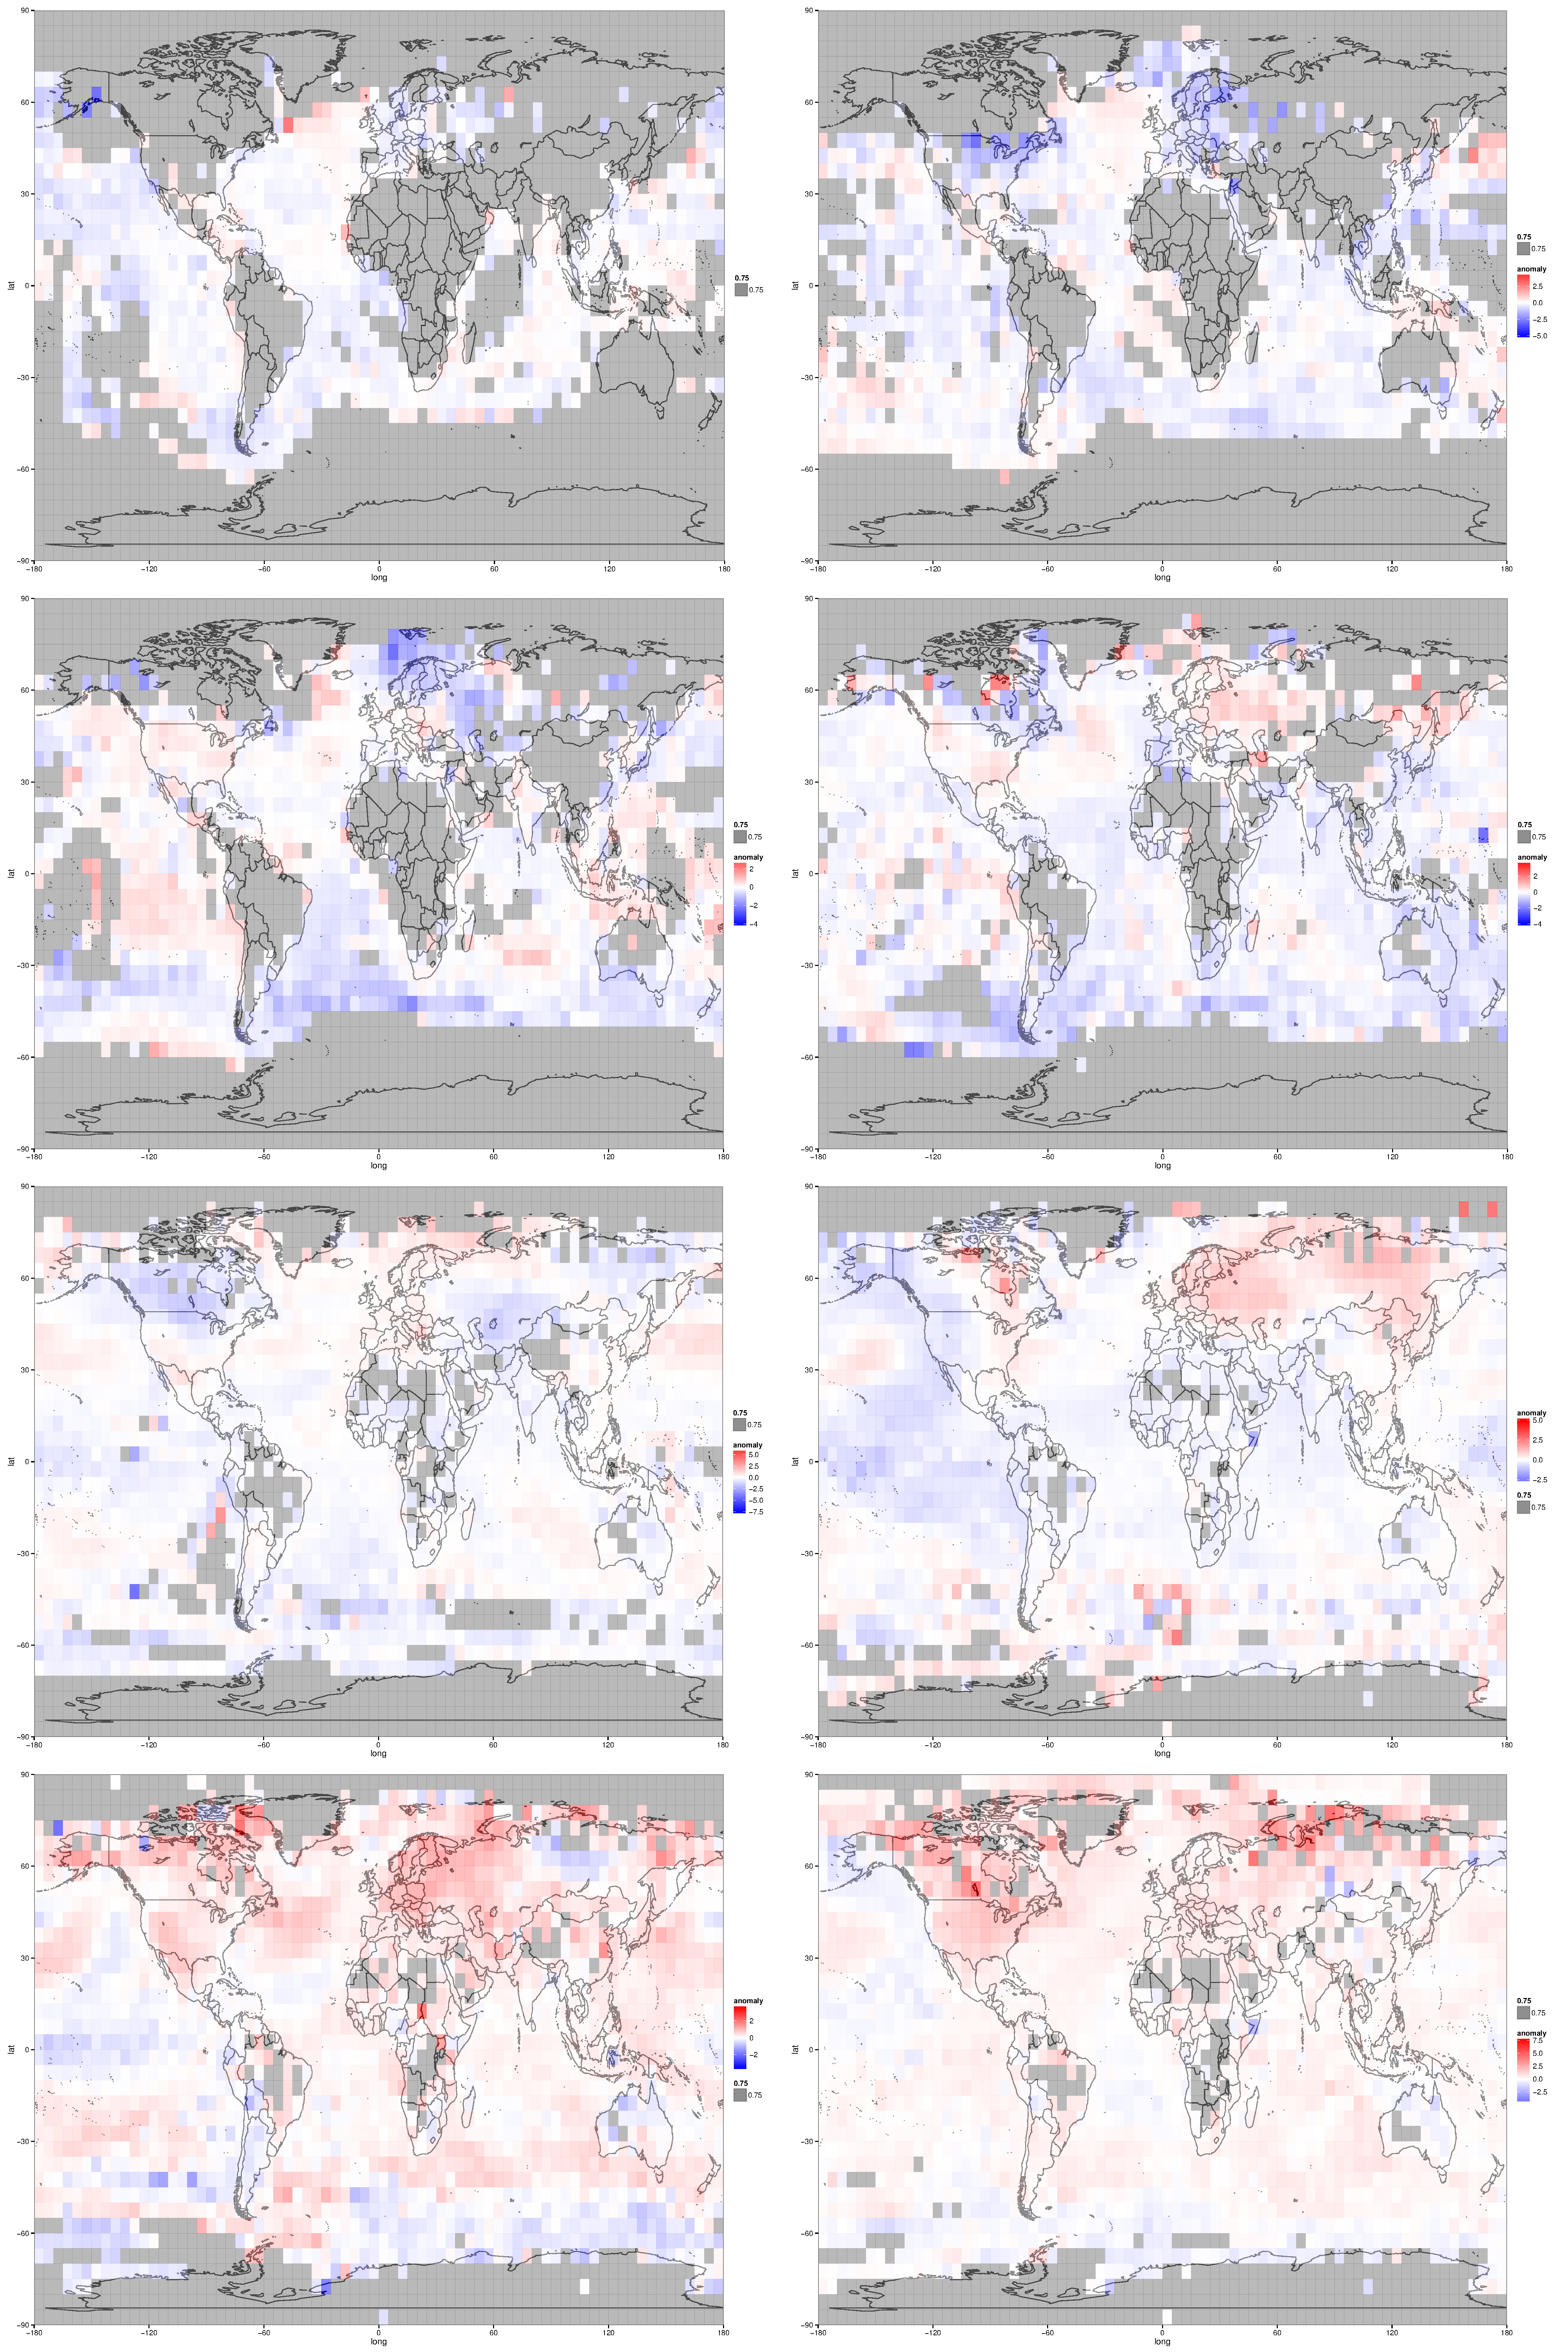
\includegraphics[width=\linewidth]{figure/chunk2} 
\end{knitrout}

\end{figure}

However, as time passes, the interior of the continents are filled in more until 2012, when only the most remote and uninhabitable areas are neglected, such as the Sahara and the polar regions.

\subsection*{Anomalies vs. Absolute Temperature}
The data presented here are recorded with respect to the 1961-1990 period.  The 1961-1990 period was chosen by the researchers who created this data set since it has some of most consistent data in terms of complete coverage of temperature values. For each station used, the baseline average over 1961-1990 was computed in order to record temperature anomalies by that station per month.

This is good for a few reasons of comparability:
\begin{enumerate}
\item Different stations are in different locations
\item Different stations use different recording methods (land vs. sea stations)
\item Different countries use different methods of calculating average monthly temperature
\end{enumerate}
Taken together, using temperature anomalies allows for comparability between the locations.

The graph below gives the overall deviation in degrees from the 1961 to 1990 trend line by month. Points plotted below zero represent an average temperature below the 1961 to 1990 trend and points plotted above zero represents an average temperature above the trend line. As can be seen, the vast majority of months from 1850 to 1950 have negative deviations indicating that temperatures from that time period were slightly cooler than the trend of temperatures from 1961 to 1990. Starting around the 1970's to 1980's most of the anomalies start to increase such that by 2010 the temperature anomoly is hoving at about 0.5 degrees above the 1961 to 1990 trend line.

\begin{knitrout}
\definecolor{shadecolor}{rgb}{0.969, 0.969, 0.969}\color{fgcolor}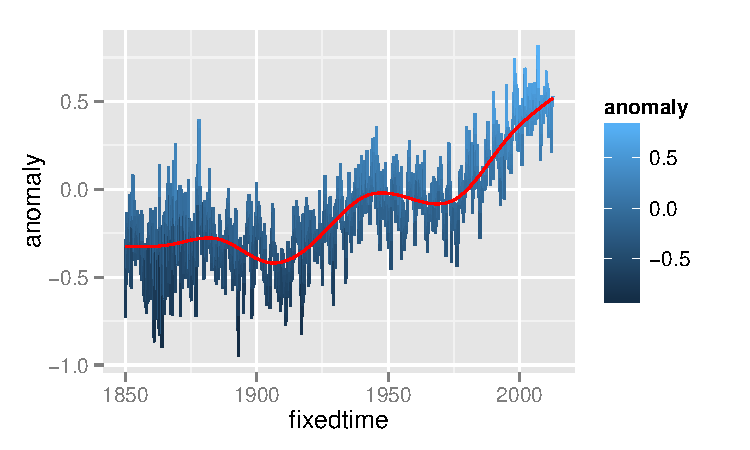
\includegraphics[width=\linewidth]{figure/plot-trend} 
\end{knitrout}


Over the past 16 years, there has been a general plateau in the increase in global temperatures that has been occuring over the past century. As can been by the fitted linear line below, the line is relatively flat indicating that no significant amount of warming has occurred globally over the past 16 years. Some skeptics have pointed to this stagnant trend of no temperature increase as evidence that we should not worry about the effects of climate change. However, we would like to point out that warming may return in the future. Further, even though we are currently in a trend of stagnating temperatures, we are not seeing any decrease in the overall temperature trend. Meaning that we are still living with the increased temperatures from previous warming periods during the twentieth century.


\begin{knitrout}
\definecolor{shadecolor}{rgb}{0.969, 0.969, 0.969}\color{fgcolor}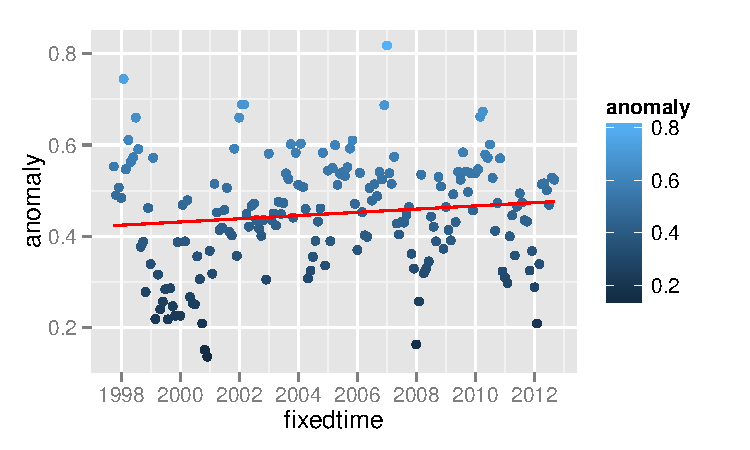
\includegraphics[width=\linewidth]{figure/15-years} 
\end{knitrout}


Indeed, if we were to extend the range back to 1975, we would see a much different picture of warming trends. A linear line over the 1975-2012 period sees a much larger increase in temperature due to the warming period during 1978-1997.

\begin{knitrout}
\definecolor{shadecolor}{rgb}{0.969, 0.969, 0.969}\color{fgcolor}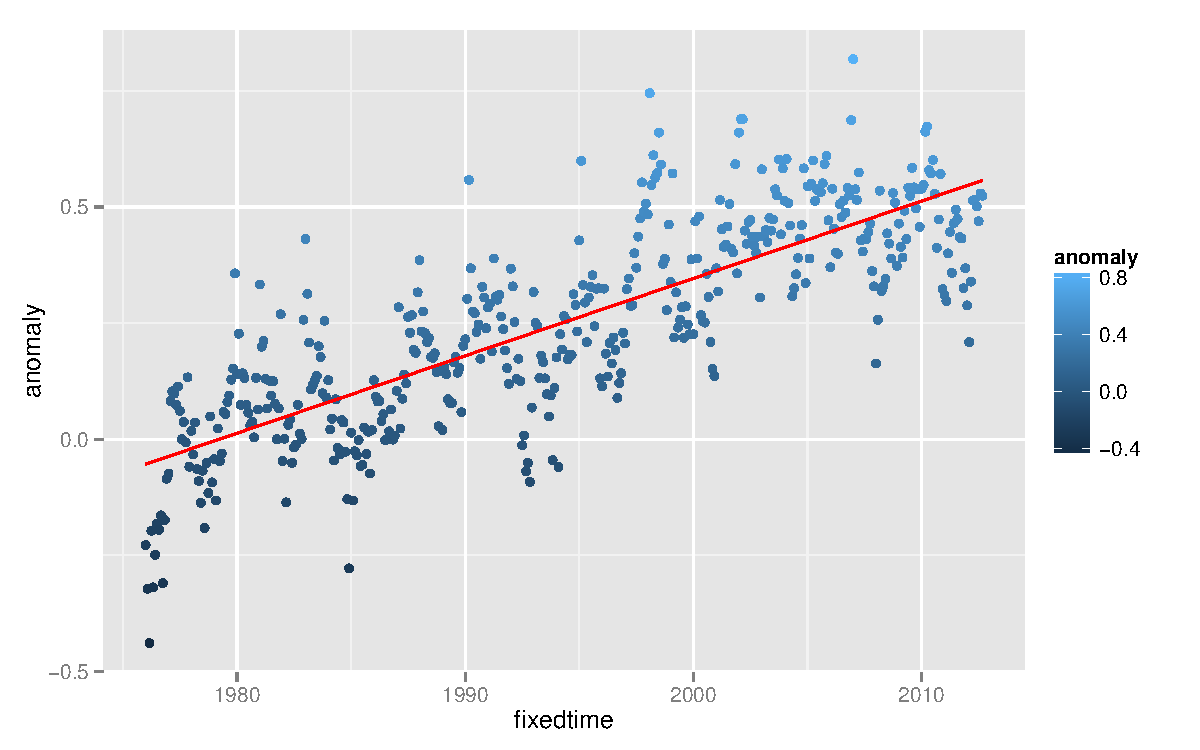
\includegraphics[width=\linewidth]{figure/recent-trend} 
\end{knitrout}


After looking at global temperature trends, we decided it would be interesting to check out trends in certain locations of interest. As such, we decided to look into the temperature data for Story County.

One general thing for this graph that is true for all the other graphs of individual locations, is that the range of anomalies is much higher than that of the global anomoly graph. Almost all of the anomolies for the global anomoly graph fell within one degree Celcius of the 1960-1991 trend. Whereas, for Story county, the majority of anomolies fall within 10 degrees Celsius of it's own 1960-1991 trend. We see from the smoothed line that the trend of anomolies has been increasing over time, indicating that Story County has risen in temperature over the past century and a half.

%Latitude and longitude for story county is at 42.0242? N, 93.5287? W
% This is lat=40 and long=-95 in our dataset
%Latitude and longitude for Augsburg Germany is 48.3647? N, 10.8953? E
% closest is lat=50 and long=10

\begin{knitrout}
\definecolor{shadecolor}{rgb}{0.969, 0.969, 0.969}\color{fgcolor}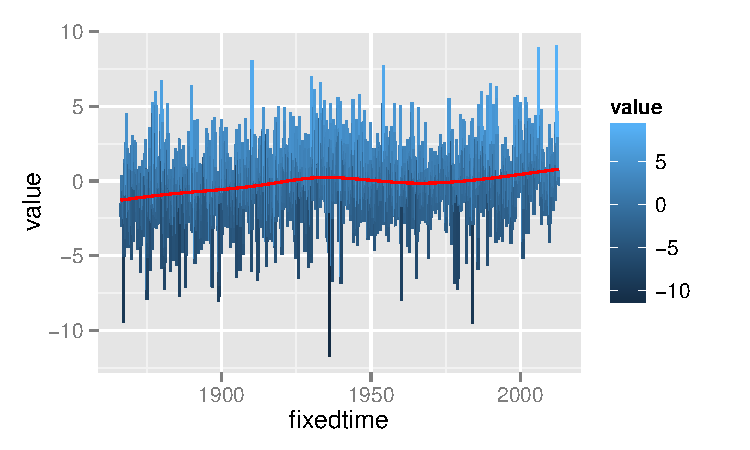
\includegraphics[width=\linewidth]{figure/story-trend} 
\end{knitrout}


The trend for Augsburg, Germany is also increasing over time. However, as compared to Story County, Augsburg has had more months with large negative anomalies as compared to large positive anomalies.

\begin{knitrout}
\definecolor{shadecolor}{rgb}{0.969, 0.969, 0.969}\color{fgcolor}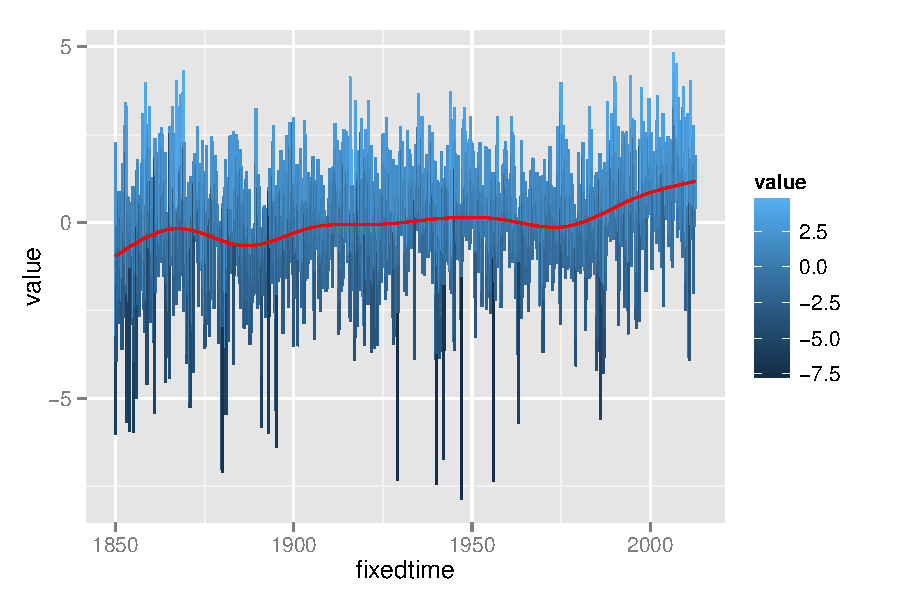
\includegraphics[width=\linewidth]{figure/augsburg-trend} 
\end{knitrout}



%Chose point in Antartica that actually had data values lat==-75 & long==15

To look at the polar regions, we choose a point with a latitude of 75 degrees South and 15 degrees East. Again, the polor region here is experiencing a warming trend.


\begin{knitrout}
\definecolor{shadecolor}{rgb}{0.969, 0.969, 0.969}\color{fgcolor}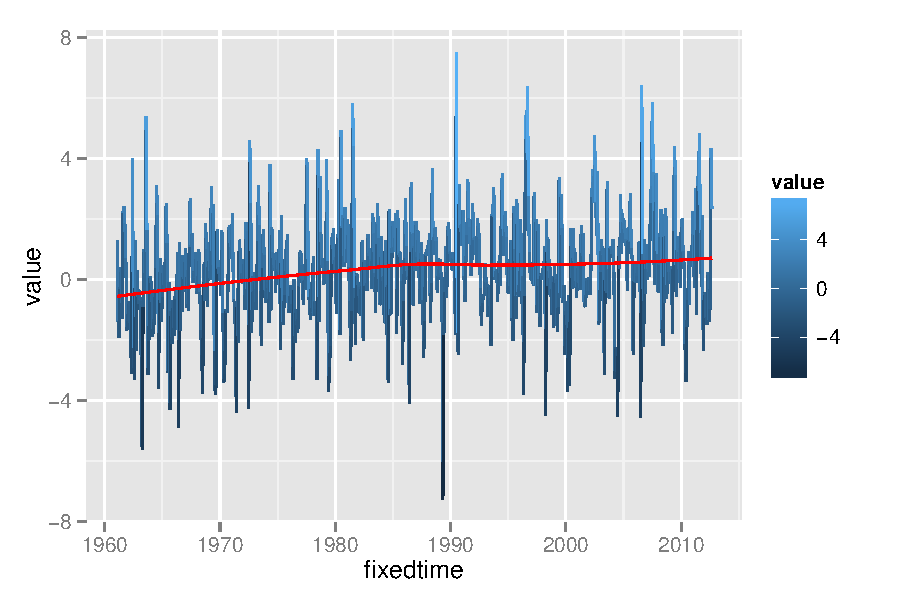
\includegraphics[width=\linewidth]{figure/antartic-trend} 
\end{knitrout}



Next, we found some interesting maps of the world colored by anomaly. Note that not every grid point has an entry and that not every grid point is greater than 0. An interesting comparison in time is between 1978 and 1997 which marked the beginning and conclusion of a substantial warming period during the twentient century. As can be noted in the 1978 map, a significantly larger portion of the map is shaded in blue, while in the 1997 those blue areas change to a neutral white. 


\begin{knitrout}
\definecolor{shadecolor}{rgb}{0.969, 0.969, 0.969}\color{fgcolor}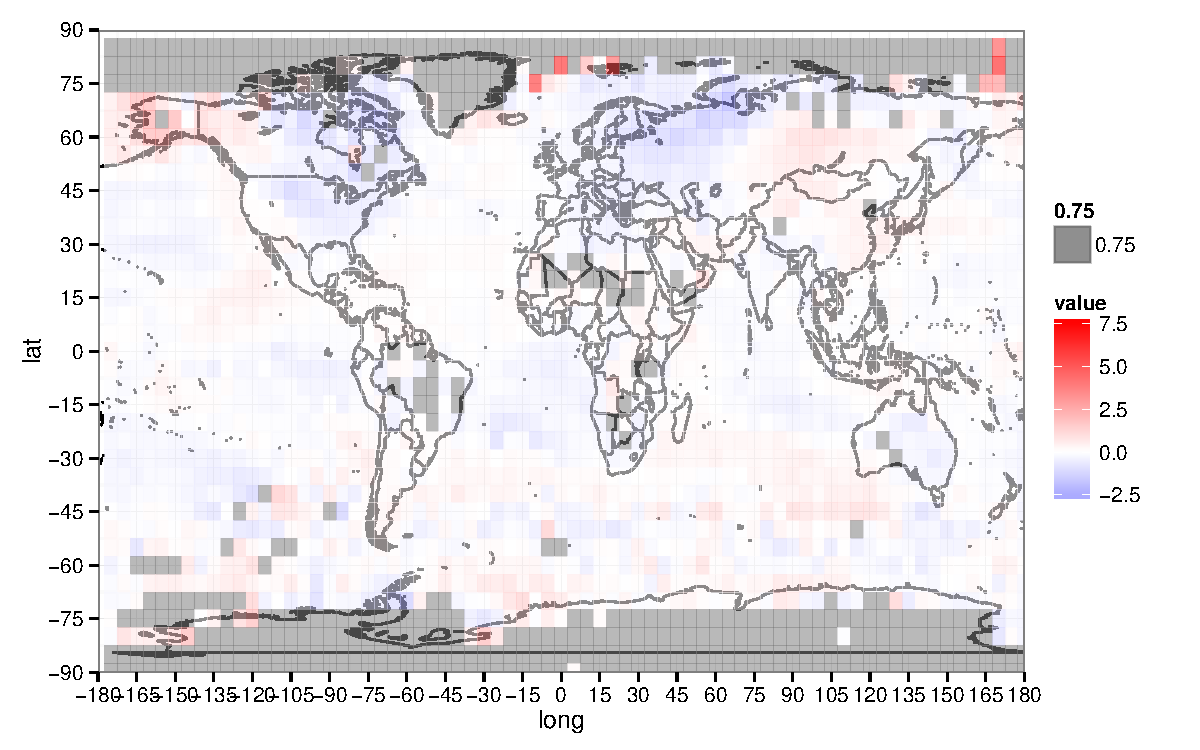
\includegraphics[width=\linewidth]{figure/1978-map} 
\end{knitrout}




\begin{knitrout}
\definecolor{shadecolor}{rgb}{0.969, 0.969, 0.969}\color{fgcolor}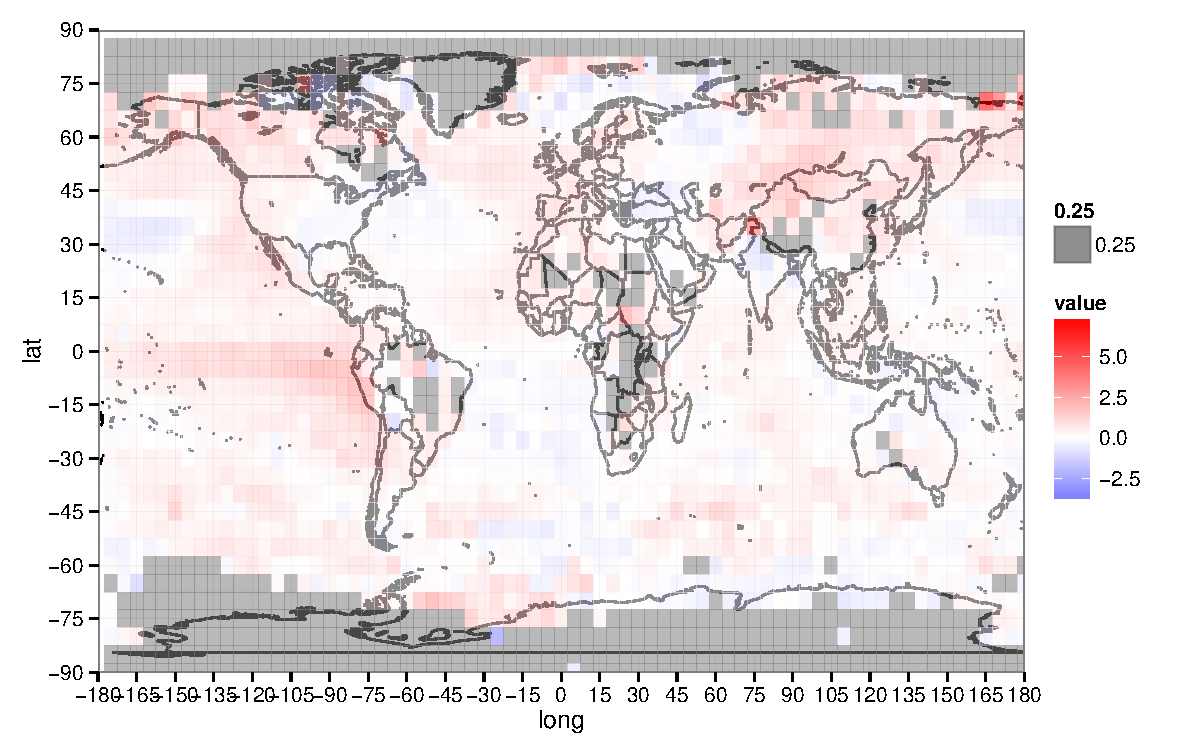
\includegraphics[width=\linewidth]{figure/1997-map} 
\end{knitrout}





\section{Conclusion:}
There will be some kind of conclusion.
\end{document}
